% Generated by code/needham.py -- do not edit by hand.
\definecolor{qocA}{rgb}{0.00,0.45,0.70}
\definecolor{qocB}{rgb}{0.90,0.60,0.00}
\definecolor{qocC}{rgb}{0.00,0.62,0.45}
\definecolor{qocD}{rgb}{0.80,0.40,0.00}
\definecolor{qocE}{rgb}{0.80,0.60,0.70}
\definecolor{qocF}{rgb}{0.35,0.70,0.90}
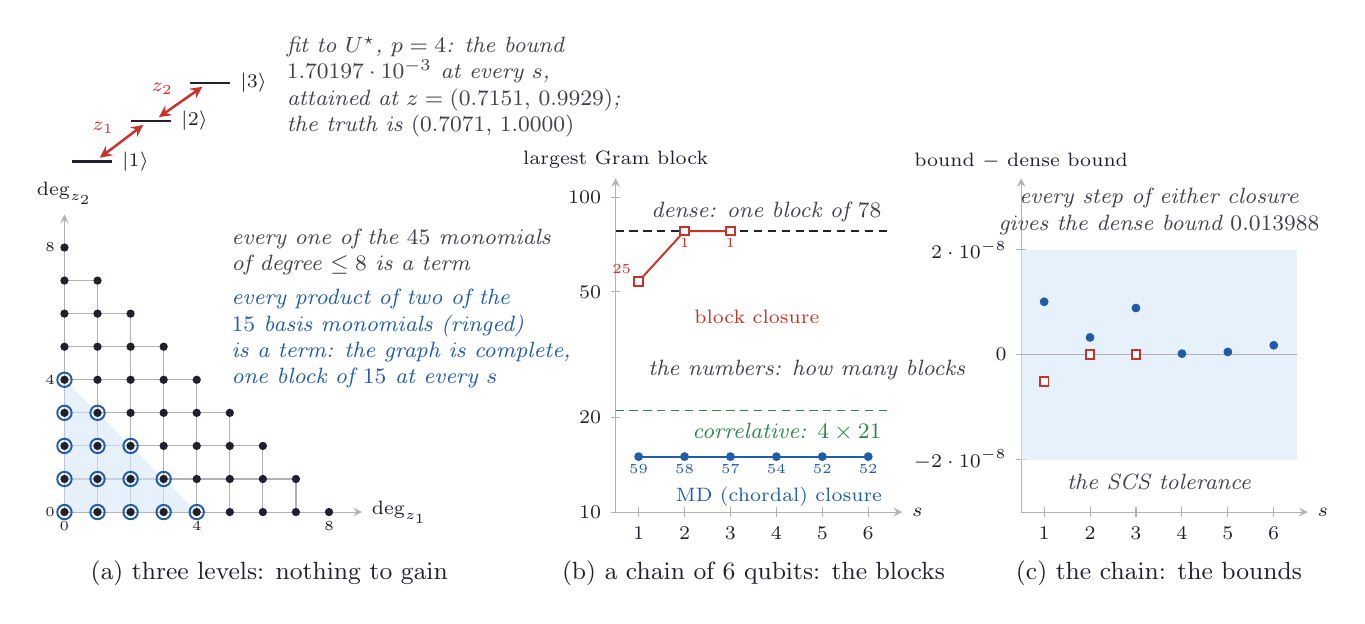
\begin{tikzpicture}[ink/.style={line width=0.9pt, ndInk}, faint/.style={line width=0.4pt, ndInk!35}, dashedink/.style={line width=0.5pt, ndInk!55, dash pattern=on 2.5pt off 2pt}, vec/.style={->, >=stealth, line width=1.2pt}, note/.style={font=\footnotesize\itshape, text=ndInk!85, align=center}, pointer/.style={->, >=stealth, line width=0.4pt, ndInk!60, shorten >=2pt, shorten <=1pt}, dot/.style={circle, fill=ndInk, inner sep=0pt, minimum size=3.4pt}, wash/.style={fill=ndSky, fill opacity=0.55}, every node/.style={text=ndInk}]
\definecolor{ndInk}{rgb}{0.13,0.13,0.18}
\definecolor{ndPaper}{rgb}{0.99,0.96,0.88}
\definecolor{ndSky}{rgb}{0.84,0.91,0.98}
\definecolor{ndRose}{rgb}{0.98,0.86,0.84}
\definecolor{ndBlue}{rgb}{0.13,0.36,0.66}
\definecolor{ndRed}{rgb}{0.78,0.20,0.16}
\definecolor{ndGold}{rgb}{0.88,0.62,0.10}
\definecolor{ndGreen}{rgb}{0.18,0.52,0.30}
\draw[faint] (0.600,0.000) -- (3.960,0.000);
\draw[faint] (0.600,0.000) -- (0.600,3.360);
\draw[faint] (0.600,0.420) -- (3.540,0.420);
\draw[faint] (1.020,0.000) -- (1.020,2.940);
\draw[faint] (0.600,0.840) -- (3.120,0.840);
\draw[faint] (1.440,0.000) -- (1.440,2.520);
\draw[faint] (0.600,1.260) -- (2.700,1.260);
\draw[faint] (1.860,0.000) -- (1.860,2.100);
\draw[faint] (0.600,1.680) -- (2.280,1.680);
\draw[faint] (2.280,0.000) -- (2.280,1.680);
\draw[faint] (0.600,2.100) -- (1.860,2.100);
\draw[faint] (2.700,0.000) -- (2.700,1.260);
\draw[faint] (0.600,2.520) -- (1.440,2.520);
\draw[faint] (3.120,0.000) -- (3.120,0.840);
\draw[faint] (0.600,2.940) -- (1.020,2.940);
\draw[faint] (3.540,0.000) -- (3.540,0.420);
\draw[faint] (0.600,3.360) -- (0.600,3.360);
\draw[faint] (3.960,0.000) -- (3.960,0.000);
\draw[faint, ->, >=stealth] (0.600,0.000) -- (4.380,0.000) node[right, font=\scriptsize] {$\deg_{z_1}$};
\draw[faint, ->, >=stealth] (0.600,0.000) -- (0.600,3.780) node[above, font=\scriptsize] {$\deg_{z_2}$};
\fill[ndSky, fill opacity=0.6] (0.600,0.000) -- (2.280,0.000) -- (0.600,1.680) -- cycle;
\fill[ndInk] (2.280,0.000) circle (1.5pt);
\fill[ndInk] (1.440,0.000) circle (1.5pt);
\fill[ndInk] (3.120,0.000) circle (1.5pt);
\fill[ndInk] (2.280,0.840) circle (1.5pt);
\fill[ndInk] (1.860,0.000) circle (1.5pt);
\fill[ndInk] (2.700,0.000) circle (1.5pt);
\fill[ndInk] (1.860,0.840) circle (1.5pt);
\fill[ndInk] (1.860,0.420) circle (1.5pt);
\fill[ndInk] (2.700,0.420) circle (1.5pt);
\fill[ndInk] (1.860,1.260) circle (1.5pt);
\fill[ndInk] (0.600,0.000) circle (1.5pt);
\fill[ndInk] (1.440,0.840) circle (1.5pt);
\fill[ndInk] (1.020,0.000) circle (1.5pt);
\fill[ndInk] (1.020,0.840) circle (1.5pt);
\fill[ndInk] (1.020,0.420) circle (1.5pt);
\fill[ndInk] (1.020,1.260) circle (1.5pt);
\fill[ndInk] (3.960,0.000) circle (1.5pt);
\fill[ndInk] (3.120,0.840) circle (1.5pt);
\fill[ndInk] (3.540,0.000) circle (1.5pt);
\fill[ndInk] (2.700,0.840) circle (1.5pt);
\fill[ndInk] (3.540,0.420) circle (1.5pt);
\fill[ndInk] (2.700,1.260) circle (1.5pt);
\fill[ndInk] (2.280,1.680) circle (1.5pt);
\fill[ndInk] (1.860,1.680) circle (1.5pt);
\fill[ndInk] (1.860,2.100) circle (1.5pt);
\fill[ndInk] (1.440,0.420) circle (1.5pt);
\fill[ndInk] (2.280,0.420) circle (1.5pt);
\fill[ndInk] (1.440,1.260) circle (1.5pt);
\fill[ndInk] (3.120,0.420) circle (1.5pt);
\fill[ndInk] (2.280,1.260) circle (1.5pt);
\fill[ndInk] (1.440,1.680) circle (1.5pt);
\fill[ndInk] (1.440,2.100) circle (1.5pt);
\fill[ndInk] (1.440,2.520) circle (1.5pt);
\fill[ndInk] (1.020,1.680) circle (1.5pt);
\fill[ndInk] (1.020,2.520) circle (1.5pt);
\fill[ndInk] (1.020,2.100) circle (1.5pt);
\fill[ndInk] (0.600,0.840) circle (1.5pt);
\fill[ndInk] (0.600,1.680) circle (1.5pt);
\fill[ndInk] (0.600,0.420) circle (1.5pt);
\fill[ndInk] (0.600,1.260) circle (1.5pt);
\fill[ndInk] (0.600,2.520) circle (1.5pt);
\fill[ndInk] (0.600,2.100) circle (1.5pt);
\fill[ndInk] (0.600,3.360) circle (1.5pt);
\fill[ndInk] (0.600,2.940) circle (1.5pt);
\fill[ndInk] (1.020,2.940) circle (1.5pt);
\draw[ndBlue, line width=0.7pt] (0.600,0.000) circle (2.6pt);
\draw[ndBlue, line width=0.7pt] (0.600,0.420) circle (2.6pt);
\draw[ndBlue, line width=0.7pt] (0.600,0.840) circle (2.6pt);
\draw[ndBlue, line width=0.7pt] (0.600,1.260) circle (2.6pt);
\draw[ndBlue, line width=0.7pt] (0.600,1.680) circle (2.6pt);
\draw[ndBlue, line width=0.7pt] (1.020,0.000) circle (2.6pt);
\draw[ndBlue, line width=0.7pt] (1.020,0.420) circle (2.6pt);
\draw[ndBlue, line width=0.7pt] (1.020,0.840) circle (2.6pt);
\draw[ndBlue, line width=0.7pt] (1.020,1.260) circle (2.6pt);
\draw[ndBlue, line width=0.7pt] (1.440,0.000) circle (2.6pt);
\draw[ndBlue, line width=0.7pt] (1.440,0.420) circle (2.6pt);
\draw[ndBlue, line width=0.7pt] (1.440,0.840) circle (2.6pt);
\draw[ndBlue, line width=0.7pt] (1.860,0.000) circle (2.6pt);
\draw[ndBlue, line width=0.7pt] (1.860,0.420) circle (2.6pt);
\draw[ndBlue, line width=0.7pt] (2.280,0.000) circle (2.6pt);
\node[font=\tiny, below] at (0.600,0.000) {$0$};
\node[font=\tiny, left] at (0.600,0.000) {$0$};
\node[font=\tiny, below] at (2.280,0.000) {$4$};
\node[font=\tiny, left] at (0.600,1.680) {$4$};
\node[font=\tiny, below] at (3.960,0.000) {$8$};
\node[font=\tiny, left] at (0.600,3.360) {$8$};
\node[note, anchor=west, align=left] at (2.600,3.300) {every one of the $45$ monomials\\ of degree $\le8$ is a term};
\node[note, anchor=west, align=left, text=ndBlue] at (2.600,2.200) {every product of two of the\\ $15$ basis monomials (ringed)\\ is a term: the graph is complete,\\ one block of $15$ at every $s$};
\draw[ink] (0.700,4.450) -- (1.200,4.450) node[right, font=\scriptsize] {$|1\rangle$};
\draw[ink] (1.450,4.966) -- (1.950,4.966) node[right, font=\scriptsize] {$|2\rangle$};
\draw[ink] (2.200,5.450) -- (2.700,5.450) node[right, font=\scriptsize] {$|3\rangle$};
\draw[<->, >=stealth, ndRed, line width=0.9pt] (1.050,4.500) -- node[above left=-1pt, font=\scriptsize, text=ndRed] {$z_1$} (1.600,4.916);
\draw[<->, >=stealth, ndRed, line width=0.9pt] (1.800,5.016) -- node[above left=-1pt, font=\scriptsize, text=ndRed] {$z_2$} (2.350,5.400);
\node[note, anchor=west, align=left] at (3.300,5.400) {fit to $U^\star$, $p=4$: the bound\\ $1.70197\cdot10^{-3}$ at every $s$,\\ attained at $z=(0.7151,\,0.9929)$;\\ the truth is $(0.7071,\,1.0000)$};
\node[font=\small, anchor=north] at (3.200,-0.500) {(a) three levels: nothing to gain};
\draw[faint, ->, >=stealth] (7.600,0.000) -- (11.240,0.000) node[right, text=ndInk] {{\scriptsize $s$}};
\draw[faint, ->, >=stealth] (7.600,0.000) -- (7.600,4.240) node[above, text=ndInk] {{\scriptsize largest Gram block}};
\draw[faint] (7.892,0.060) -- (7.892,-0.060) node[below, font=\scriptsize, text=ndInk] {$1$};
\draw[faint] (8.475,0.060) -- (8.475,-0.060) node[below, font=\scriptsize, text=ndInk] {$2$};
\draw[faint] (9.058,0.060) -- (9.058,-0.060) node[below, font=\scriptsize, text=ndInk] {$3$};
\draw[faint] (9.642,0.060) -- (9.642,-0.060) node[below, font=\scriptsize, text=ndInk] {$4$};
\draw[faint] (10.225,0.060) -- (10.225,-0.060) node[below, font=\scriptsize, text=ndInk] {$5$};
\draw[faint] (10.808,0.060) -- (10.808,-0.060) node[below, font=\scriptsize, text=ndInk] {$6$};
\draw[faint] (7.660,0.000) -- (7.540,0.000) node[left, font=\scriptsize, text=ndInk] {$10$};
\draw[faint] (7.660,1.204) -- (7.540,1.204) node[left, font=\scriptsize, text=ndInk] {$20$};
\draw[faint] (7.660,2.796) -- (7.540,2.796) node[left, font=\scriptsize, text=ndInk] {$50$};
\draw[faint] (7.660,4.000) -- (7.540,4.000) node[left, font=\scriptsize, text=ndInk] {$100$};
\draw[line width=0.9pt, ndInk, dash pattern=on 3pt off 2pt] (7.600,3.568) -- (11.100,3.568);
\draw[line width=0.6pt, ndGreen, dash pattern=on 3pt off 2pt] (7.600,1.289) -- (11.100,1.289);
\node[note, anchor=south east] at (11.100,3.568) {dense: one block of $78$};
\node[note, anchor=north east, text=ndGreen] at (11.100,1.249) {correlative: $4\times21$};
\draw[line width=0.7pt, ndBlue] (7.892,0.704) -- (8.475,0.704) -- (9.058,0.704) -- (9.642,0.704) -- (10.225,0.704) -- (10.808,0.704);
\fill[ndBlue] (7.892,0.704) circle (1.6pt);
\fill[ndBlue] (8.475,0.704) circle (1.6pt);
\fill[ndBlue] (9.058,0.704) circle (1.6pt);
\fill[ndBlue] (9.642,0.704) circle (1.6pt);
\fill[ndBlue] (10.225,0.704) circle (1.6pt);
\fill[ndBlue] (10.808,0.704) circle (1.6pt);
\node[below, font=\tiny, text=ndBlue, inner sep=2.5pt] at (7.892,0.704) {$59$};
\node[below, font=\tiny, text=ndBlue, inner sep=2.5pt] at (8.475,0.704) {$58$};
\node[below, font=\tiny, text=ndBlue, inner sep=2.5pt] at (9.058,0.704) {$57$};
\node[below, font=\tiny, text=ndBlue, inner sep=2.5pt] at (9.642,0.704) {$54$};
\node[below, font=\tiny, text=ndBlue, inner sep=2.5pt] at (10.225,0.704) {$52$};
\node[below, font=\tiny, text=ndBlue, inner sep=2.5pt] at (10.808,0.704) {$52$};
\draw[line width=0.7pt, ndRed] (7.892,2.930) -- (8.475,3.568) -- (9.058,3.568);
\draw[ndRed, line width=0.7pt, fill=white] (7.837,2.875) rectangle (7.947,2.985);
\draw[ndRed, line width=0.7pt, fill=white] (8.420,3.513) rectangle (8.530,3.623);
\draw[ndRed, line width=0.7pt, fill=white] (9.003,3.513) rectangle (9.113,3.623);
\node[above left, font=\tiny, text=ndRed, inner sep=2.5pt] at (7.892,2.930) {$25$};
\node[below, font=\tiny, text=ndRed, inner sep=2.5pt] at (8.475,3.568) {$1$};
\node[below, font=\tiny, text=ndRed, inner sep=2.5pt] at (9.058,3.568) {$1$};
\node[font=\scriptsize, anchor=west, text=ndBlue] at (8.242,0.200) {MD (chordal) closure};
\node[font=\scriptsize, anchor=west, text=ndRed] at (8.475,2.480) {block closure};
\node[note, anchor=west] at (7.892,1.800) {the numbers: how many blocks};
\node[font=\small, anchor=north] at (9.350,-0.500) {(b) a chain of $6$ qubits: the blocks};
\draw[faint, ->, >=stealth] (12.750,0.000) -- (16.390,0.000) node[right, text=ndInk] {{\scriptsize $s$}};
\draw[faint, ->, >=stealth] (12.750,0.000) -- (12.750,4.240) node[above, text=ndInk] {{\scriptsize bound $-$ dense bound}};
\draw[faint] (13.042,0.060) -- (13.042,-0.060) node[below, font=\scriptsize, text=ndInk] {$1$};
\draw[faint] (13.625,0.060) -- (13.625,-0.060) node[below, font=\scriptsize, text=ndInk] {$2$};
\draw[faint] (14.208,0.060) -- (14.208,-0.060) node[below, font=\scriptsize, text=ndInk] {$3$};
\draw[faint] (14.792,0.060) -- (14.792,-0.060) node[below, font=\scriptsize, text=ndInk] {$4$};
\draw[faint] (15.375,0.060) -- (15.375,-0.060) node[below, font=\scriptsize, text=ndInk] {$5$};
\draw[faint] (15.958,0.060) -- (15.958,-0.060) node[below, font=\scriptsize, text=ndInk] {$6$};
\draw[faint] (12.810,0.667) -- (12.690,0.667) node[left, font=\scriptsize, text=ndInk] {$-2\cdot10^{-8}$};
\draw[faint] (12.810,2.000) -- (12.690,2.000) node[left, font=\scriptsize, text=ndInk] {$0$};
\draw[faint] (12.810,3.333) -- (12.690,3.333) node[left, font=\scriptsize, text=ndInk] {$2\cdot10^{-8}$};
\fill[ndSky, fill opacity=0.6] (12.750,0.667) rectangle (16.250,3.333);
\draw[faint] (12.750,2.000) -- (16.250,2.000);
\fill[ndBlue] (13.042,2.671) circle (1.6pt);
\fill[ndBlue] (13.625,2.218) circle (1.6pt);
\fill[ndBlue] (14.208,2.591) circle (1.6pt);
\fill[ndBlue] (14.792,2.012) circle (1.6pt);
\fill[ndBlue] (15.375,2.033) circle (1.6pt);
\fill[ndBlue] (15.958,2.118) circle (1.6pt);
\draw[ndRed, line width=0.7pt, fill=white] (12.987,1.602) rectangle (13.097,1.712);
\draw[ndRed, line width=0.7pt, fill=white] (13.570,1.945) rectangle (13.680,2.055);
\draw[ndRed, line width=0.7pt, fill=white] (14.153,1.945) rectangle (14.263,2.055);
\node[note, anchor=north] at (14.500,0.600) {the SCS tolerance};
\node[note, anchor=south, align=center] at (14.500,3.400) {every step of either closure\\ gives the dense bound $0.013988$};
\node[font=\small, anchor=north] at (14.500,-0.500) {(c) the chain: the bounds};
\end{tikzpicture}
